
%\begin{figure}[h]
%    \centering
%
%    \advance\leftskip-3.5cm
%    \advance\rightskip-4cm
%	
%	\minipage{0.30\textwidth}
%	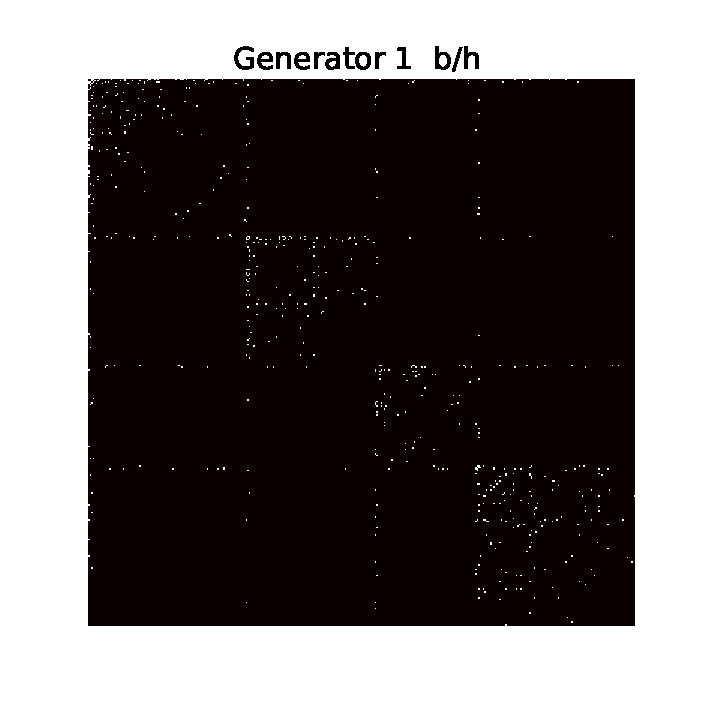
\includegraphics[scale=0.32]{img/g1}
%	\endminipage
%	\minipage{0.30\textwidth}
%	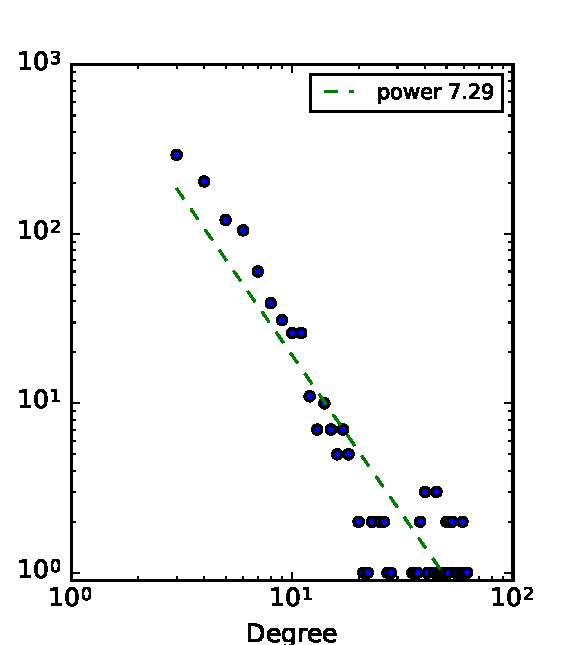
\includegraphics[scale=0.32]{img/g1_d}
%	\endminipage
%	\vspace{-0.4cm}
%	\minipage{0.30\textwidth}
%	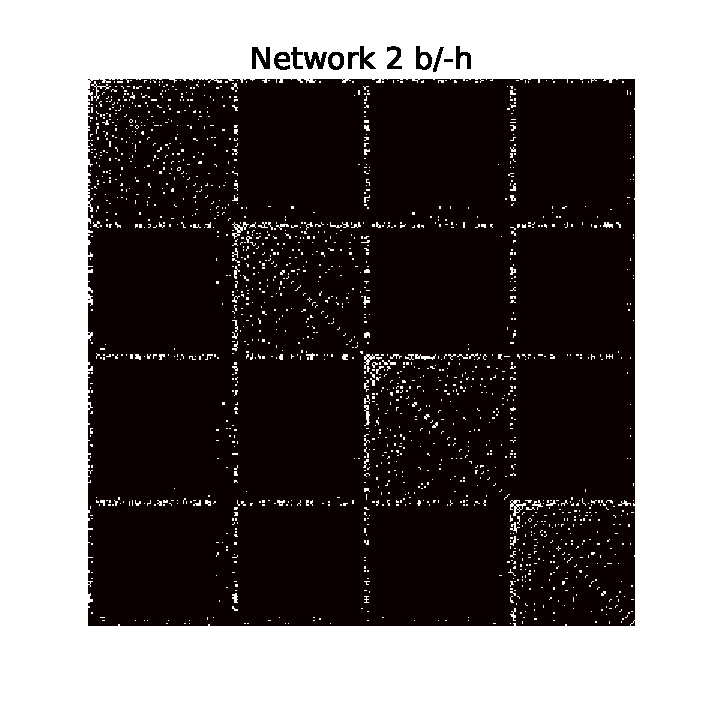
\includegraphics[scale=0.32]{img/g2}
%	\endminipage
%	\minipage{0.30\textwidth}
%	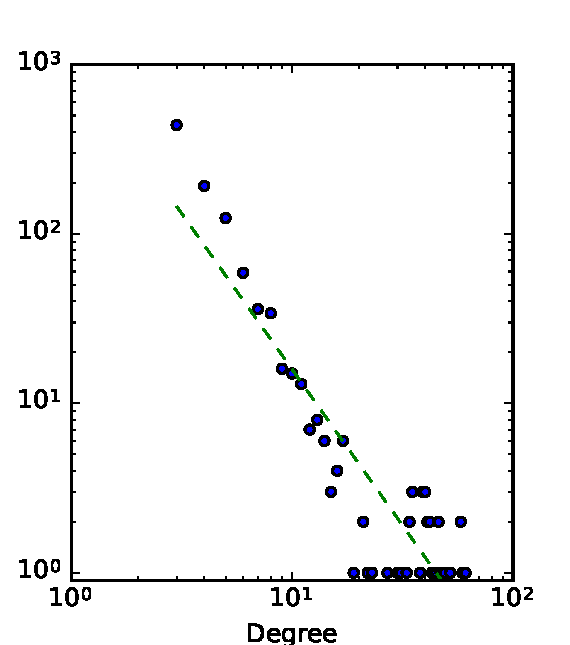
\includegraphics[scale=0.32]{img/g2_d}
%	\endminipage
%
%	%\vspace{-0.4cm}
%
%	\minipage{0.30\textwidth}
%	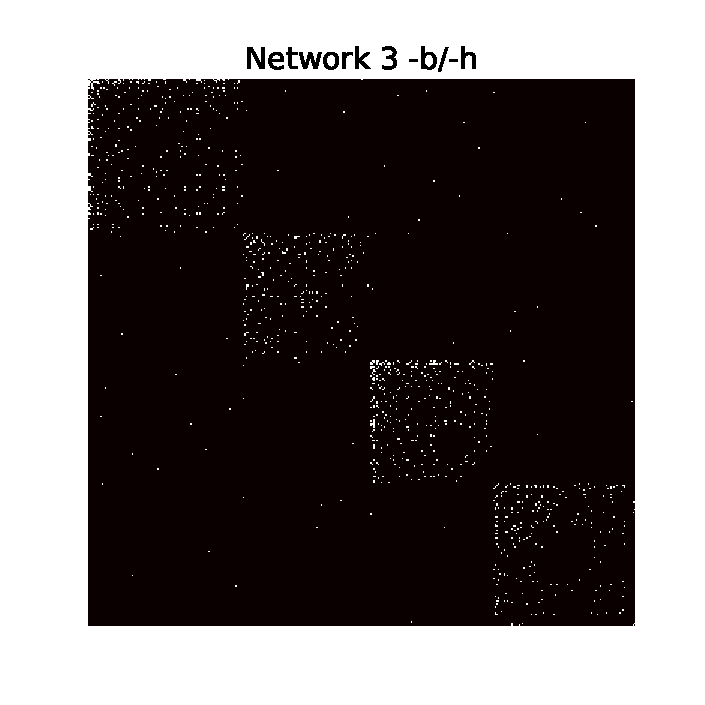
\includegraphics[scale=0.32]{img/g3}
%	\endminipage
%	\minipage{0.30\textwidth}
%	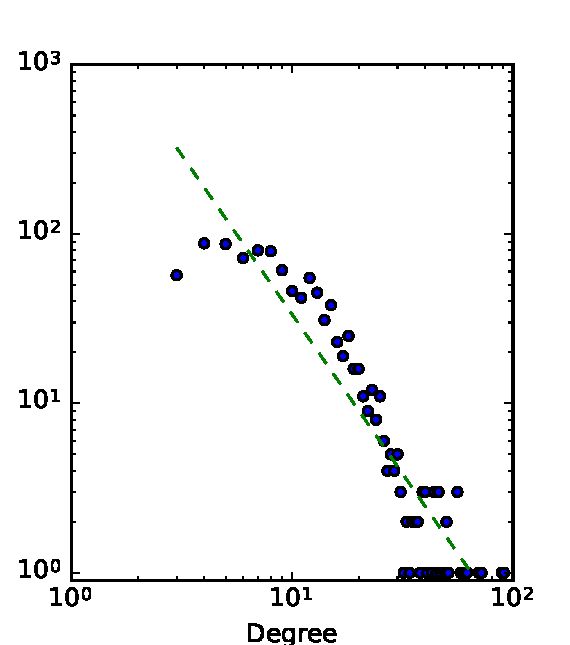
\includegraphics[scale=0.32]{img/g3_d}
%	\endminipage
%	\vspace{-0.4cm}
%	\minipage{0.30\textwidth}
%	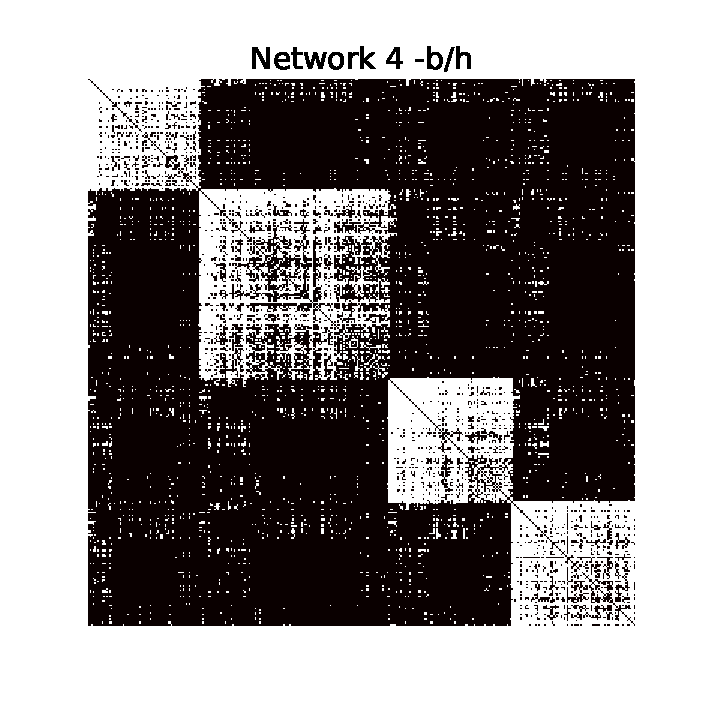
\includegraphics[scale=0.32]{img/g4}
%	\endminipage
%	\minipage{0.30\textwidth}
%	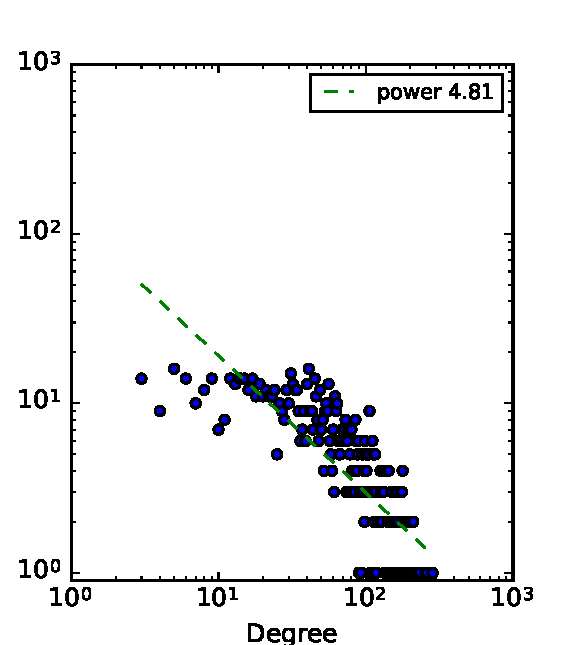
\includegraphics[scale=0.32]{img/g4_d}
%	\endminipage
%	
%	\caption{Adjacency matrices (left) and global degree distributions (right) for the artificial networks Network 1, ..,Network 4.}
%	\label{fig:synt_graph}
%\end{figure}
%
%\vspace{1cm}

\begin{figure}[h]
        \centering
        \begin{subfigure}[b]{0.480\textwidth}
            \centering
            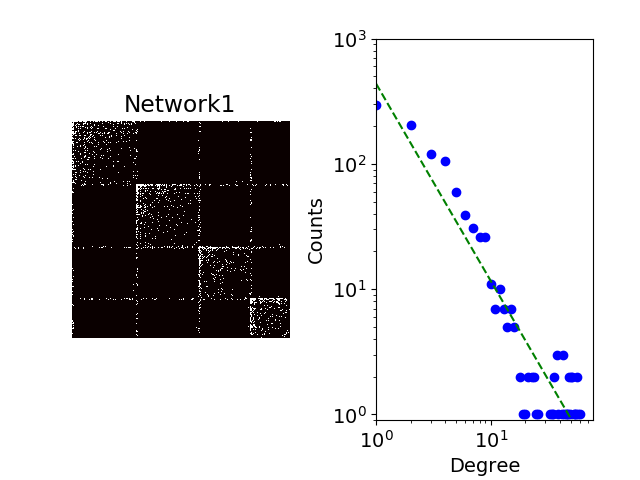
\includegraphics[width=\textwidth]{img/corpus/network1_dd}
            \caption {{\small Network 1}}    
            \label{fig:mean and std of net14}
        \end{subfigure}
        \hfill
        \begin{subfigure}[b]{0.480\textwidth}  
            \centering 
            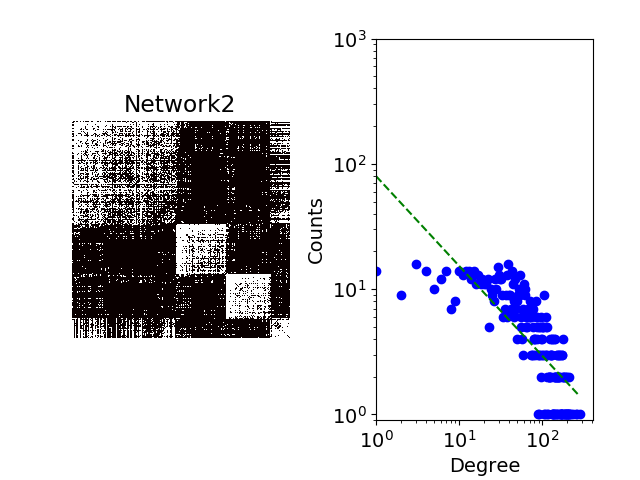
\includegraphics[width=\textwidth]{img/corpus/network2_dd}
            \caption {{\small Network 2}}    
            \label{fig:mean and std of net24}
        \end{subfigure}
        \vskip\baselineskip
        \begin{subfigure}[b]{0.480\textwidth}   
            \centering 
            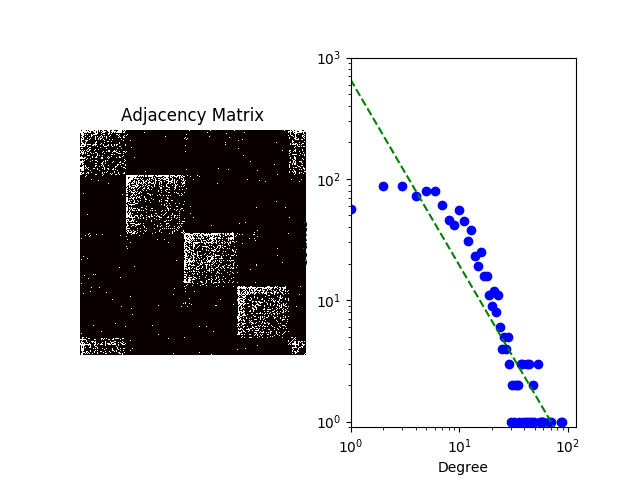
\includegraphics[width=\textwidth]{img/corpus/network3_dd}
            \caption{{\small Network 3}}    
            \label{fig:mean and std of net34}
        \end{subfigure}
        \quad
        \begin{subfigure}[b]{0.480\textwidth}   
            \centering 
            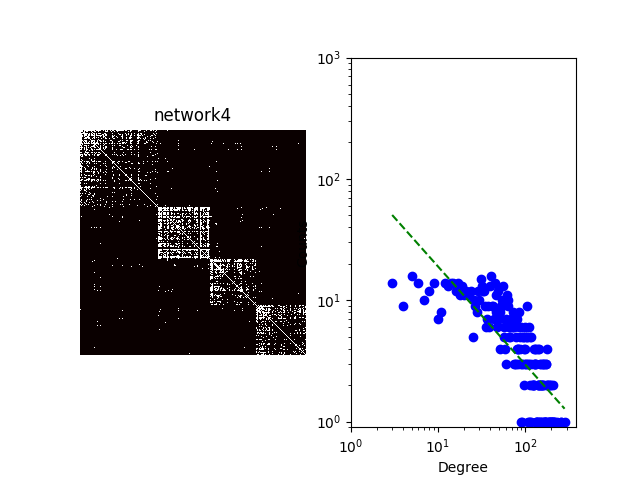
\includegraphics[width=\textwidth]{img/corpus/network4_dd}
            \caption{{\small Network 4}}    
            \label{fig:mean and std of net44}
        \end{subfigure}
	\caption{Adjacency matrices (left) and global degree distributions (right) for the artificial networks Network 1, ..,Network 4.}
	\label{fig:synt_graph}
\end{figure}
